%!TeX root=../tese.tex
%("dica" para o editor de texto: este arquivo é parte de um documento maior)
% para saber mais: https://tex.stackexchange.com/q/78101

\chapter{Modelo de Aprendizado}
\label{chap:modelo}

O objetivo deste capítulo é apresentar as definições dos modelos de aprendizado de W-operadores multicamadas (WOMC) nos contextos de transformação de imagens e para classificação de imagens, de acordo com o modelo proposto por \cite{DIEGO:01}, que serão a base de desenvolvimento deste trabalho.


\section{W-operadores Multicamadas para Transformação de Imagens}
\label{sec:Wop_transformacao}

No contexto de transformação de imagens, os WOMC são uma composição de $n$ W-operadores aplicados em sequência a uma imagem de entrada $X \in \mathcal{P}\left( E \right)$ conforme apresentado em \ref{subsec:compwop}.

A família de W-operadores considerada neste trabalho é caracterizada por janelas com dimensão máxima fixada. Seja $d_{W} \geq 3$ um número ímpar e $F_{d_{W}} = \left\{ - \left( d_{W} -1 \right) /2 ,..., \left(	d_{W} - 1 \right) /2 \right\}^{2} $ o quadrado de lado $d_{W}$ centrado na origem de $E$. Nós consideramos que a janela $W$ de cada W-operador de um WOMC é um subconjunto de $F_{d_{W}}$, com a restrição de ser um conjunto conectado, ou seja, para cada $w, w' \in W$ existe uma sequência $w_{0},...,w_{r} \in W, \ r \geq 1, $ tal que $w_{0} = w, \ w_{r} = w' $ e 
$$ \| w_{i} - w_{i+1} \|_{\infty} = 1, \text{ para todo } i=0,...,r-1. $$
Formalmente, $W \in \mathscr{C}$ em que
$$ \mathscr{C} = \left\{ W \subseteq F_{d_{W}}  : W \text{ é conectado} \right\}. $$
Na figura \ref{fig:wconect} apresentamos exemplos de janelas que estão e não estão em $\mathscr{C}$.

\begin{figure}
  \centering

  \begin{subfigure}{0.4\textwidth}
    \centering
    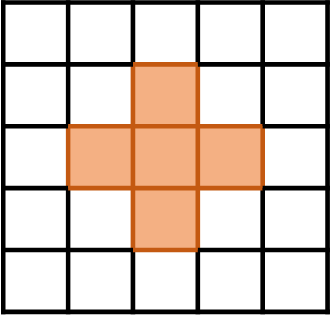
\includegraphics[width=.8\textwidth]{figuras/W_conectada.png}
    \caption{Janela $W \in \mathscr{C}$ - Conectada\label{fig:subfig:wconect}}
  \end{subfigure}
  \begin{subfigure}{0.4\textwidth}
    \centering
      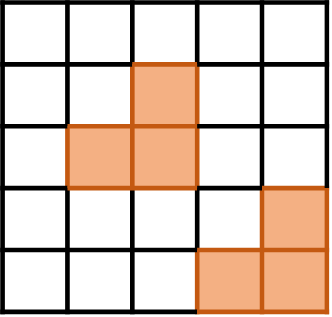
\includegraphics[width=.8\textwidth]{figuras/W_nconectada.png}
    \caption{Janela $W \notin \mathscr{C}$ - Desconectada.\label{fig:subfig:wnotconect}}
  \end{subfigure}

  \caption{Exemplo de Janelas contida em $F_{5}$ que respeita (esquerda) e não respeita (direita) a restrição de W-operadores de ser conectada.\label{fig:wconect}}
\end{figure}

Para cada $W \in \mathscr{C} $, defina o conjunto de todas as funções binárias com domínio $\left\{ 0,1 \right\}^{W} $ como
$$ \mathcal{F}_{W} = \left\{ f: \left\{ 0,1 \right\}^{W} \mapsto \left\{ 0,1 \right\} \right\}. $$
Definimos a coleção de W-operadores com janela em $ \mathscr{C}$, que são completamente definidos por $W \in \mathscr{C} $ e $f \in \mathcal{F}_{W}$, como
$$\mathcal{F} = \left\{ \left( W,f \right) : W \in \mathscr{C}, \ f \in \mathcal{F}_{W} \right\}. $$
Por fim, o produto cartesiano das $n$ cópias de $\mathcal{F}$ pode ser definido como
$$\Theta = \prod_{i=1}^{n} \mathcal{F}, $$
e um elemento $\theta$ em $\Theta$ será então uma sequência de $n$ W-operadores com janelas em $\mathscr{C}$ denotada por
$$ \theta := \left\{ \left(W_{1}, f_{\psi_{1}} \right), \cdot \cdot \cdot, \left(W_{n}, f_{\psi_{n}} \right) \right\}$$

Para cada $\theta \in \Theta$ temos o WOMC 
\begin{equation}
    \psi_{\theta} := \left( \psi_{n} \circ \cdot \cdot \cdot \circ \psi_{1}  \right).
    \label{eq:multicamadas_1}
\end{equation}
Um WOMC no contexto de transformação de imagens pode ser visto como um pipeline de transformação de imagens no qual cada W-operador executa sequencialmente uma transformação em uma imagem de entrada $X$, e uma imagem transformada $Y = \psi_{\theta} \left( X \right) $ é obtida. 

O Espaço de Hipóteses dos WOMC para a transformação de imagens será então
$$\mathcal{H} := \left\{ \psi_{\theta} : \theta \in \Theta \right\}. $$


%%%%%%%%%%%%%%%%%%%%%%%%%%%%%%%%%%%%%%%%%%%%%%%%%%%%%%%%%%%%%%%%%%%%%%%%%%

\section{W-operador Multicamadas para Classificação de Imagens}

WOMC também podem ser utilizados no contexto de classificação de imagens binárias, onde a \textit{transformação} da imagem de entrada deve levar a uma classificação ao invés de uma imagem transformada. Para isso, podemos considerar a composição de \textit{W-operadores emoldurados}, onde após a aplicação de cada operador, a imagem perde dimensões, e ao final da pipeline obtemos um número em $\left\{ 0,1 \right\}$.

\subsection{W-operadores Emoldurados}

Seja $F_{1} = \left\{ \left( 0,0 \right) \right\}$ a origem de $E = \mathbb{Z}^{2}$ e para $p \geq 3$, ímpar, seja
$$F_{p} = \left\{ - \left(p-1 \right) /2 , ... , \left( p-1 \right) /2 \right\}^{2} \subseteq E $$
o conjunto de pontos em $E$ que formam um quadrado de $p^{2}$ pontos centrados na origem. Chamamos de $F_{p}$ a moldura de tamanho $p$. Uma imagem está emoldurada em $F_{p}$ se
$$X \subseteq F_{p}.$$
Se $X$ está emoldurado em $F_{p}$, então $X$ pode ser representado como uma imagem com $p \times p$ pixels.

Ao analisar $X$, e interpretando um W-operador como centralizando a janela $W$ em cada ponto em $z \in F_{p}$ e assumindo $z \in \psi \left( X \right)$ baseado em $f_{\psi} \left( X \cap W_{z} \cap F_{p} \right)$, podemos observar que, na verdade, não podemos centralizar a janela $W$ em todos os pontos de $F_{p}$, uma vez que $W$ não está contida em $F_{p}$ se estiver centrada em pontos próximos às bordas da imagem.

A proximidade das bordas pode ser definida em termos de uma moldura que contém $W$, assumindo que $W \subseteq F_{d_{W}}, \ d_{W} \geq 3$ ímpar, ou seja, a janela $W$ é um subconjunto da moldura $d_{W}$ com $d_{W} \leq p$. Então, podemos definir o W-operador emoldurado associado a $\psi \in \Psi_{W}$ como
\begin{equation}
    \psi_{p,d_{W}}^{fr} \left( X \right) = \psi \left( X \right) \cap F_{p-(d_{W}-1)}
    \label{eq:wemoldurado}
\end{equation}
para qualquer $X \subseteq F_{p}$, que é obtido ao centralizar a janela $W$ apenas em pontos $z \in F_{p}$ no qual $ \left[ F_{d_{W}} \right]_{z} \subseteq F_{p} $, ou seja, a moldura de $W$ está completamente contida na moldura de $X$. A Figura \ref{fig:dig0jan1} apresenta um exemplo de W-operador emoldurado.

Quando $\psi_{p,d_{W}}^{fr}$ é aplicado a uma imagem emoldurada em $F_{p}$ a imagem resultante perderá $\left( d_{W}-1 \right)$ linhas e colunas, contendo $p- \left( d_{W}-1 \right) \times p- \left( d_{W}-1 \right)$ pixels e estará emoldurada em $ F_{p-(d_{W}-1)}$, portanto
$$\psi_{p,d_{W}}^{fr} : \mathcal{P} \left( F_{p} \right) \to  \mathcal{P} \left( F_{p-(d_{W}-1)} \right). $$

\begin{figure}
    \centering
    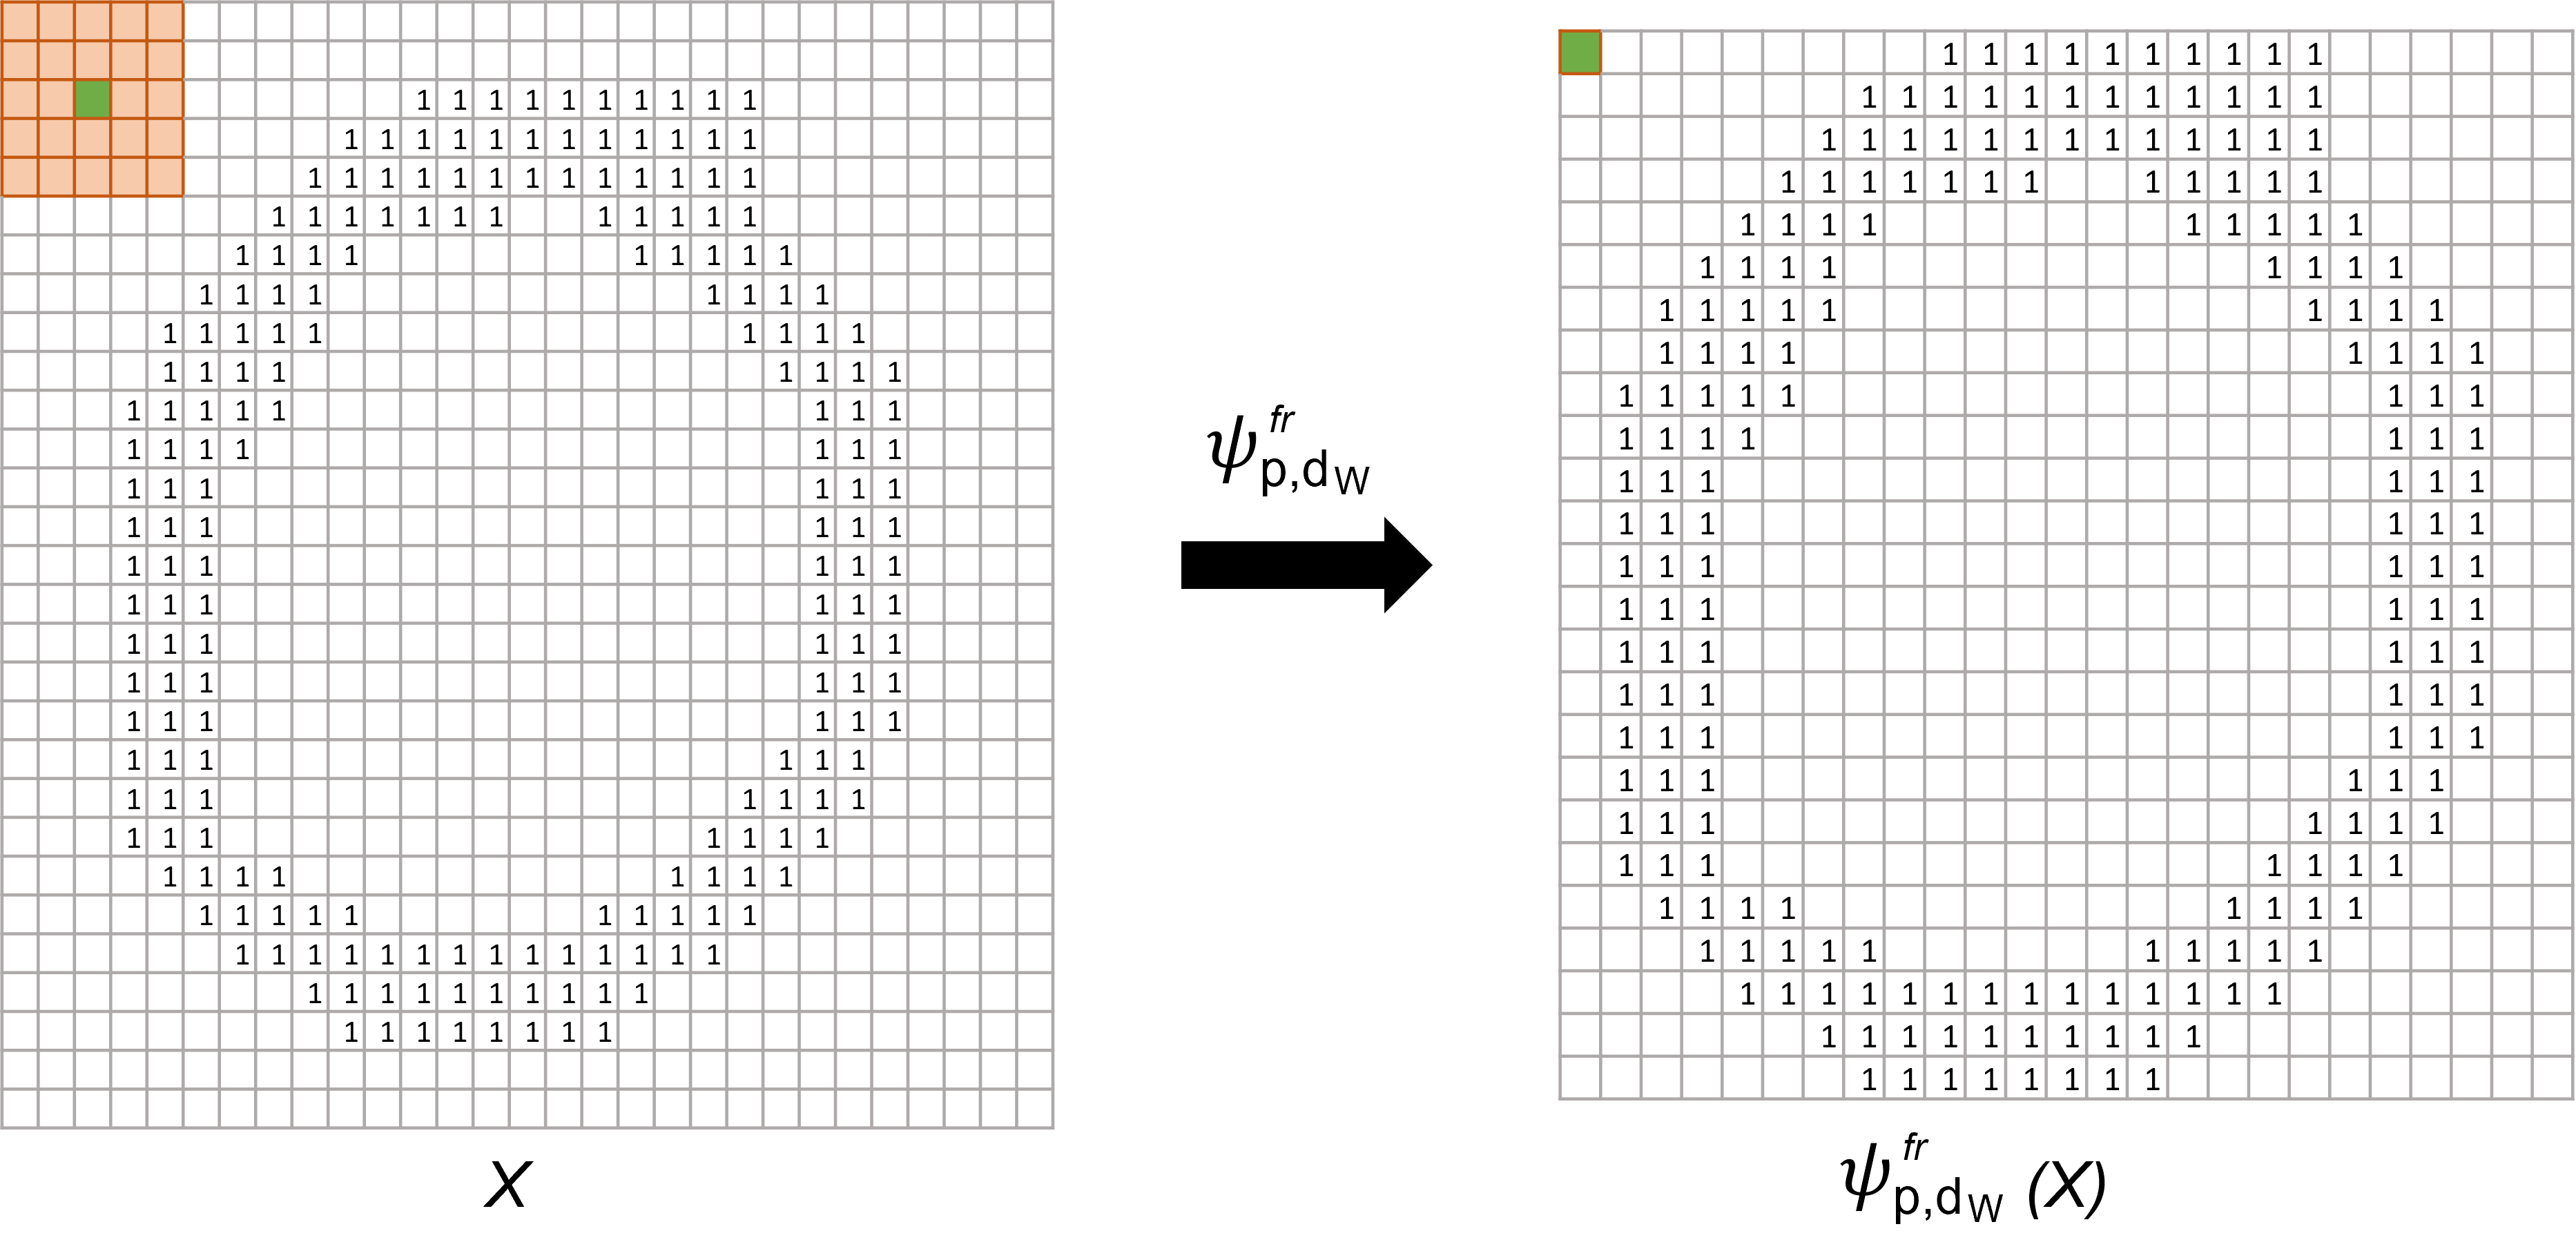
\includegraphics[scale = 0.5]{figuras/digito0_janela1_framed.png}
    \caption{Exemplo de um W-operador emoldurado $ \psi_{p,d_{W}}^{fr}$ com janela $W_{1} \subseteq F_{5}$ em laranja, na imagem $X$ a esquerda, centrado no primeiro pixel possível em verde. A imagem $ \psi_{p,d_{W}}^{fr} \left( X \right)$, obtida após aplicação do operador identidade, encontra-se a direita, com redução de dimensionalidade, indicando o pixel correspondente ao primeiro pixel de $X$ também em verde.}
    \label{fig:dig0jan1}
\end{figure}

\subsection{Classificação}

Considerando os W-operadores emoldurados definidos em \eqref{eq:wemoldurado} observamos que, como a cada aplicação de um W-operador emoldurado perdemos $d_{w} - 1$ dimensões, se aplicarmos
$$n = \left( p - 1 \right) / \left( d_{W} - 1 \right)$$
W-operadores emoldurados obteremos uma imagem com apenas um pixel, assumindo que $n \in \mathbb{Z}$ e $n \geq 2$. Dessa forma, a aplicação de $n$ W-operadores emoldurados gerará um classificador de $\mathcal{P}(F_{p})$ em $\mathcal{P}(F_{1}) \simeq \{0,1\}$.

Para cada $ \theta = \left\{ \left(W_{1}, f_{1} \right), ..., \left(W_{n}, f_{n} \right) \right\} 
\in \Theta $, seja $ \theta_{fr} = \left\{ \psi_{1}^{fr},..., \psi_{n}^{fr} \right\}$ a sequência de W-operadores emoldurados dados por
$$\psi_{i}^{fr}:= \left( \psi_{i} \right)_{p-(i-1)(d_{W}-1),d_{W}}^{fr} \left( X \right) = \psi_{i} \left(X \right) \cap F_{p-i(d_{W}-1)} $$
para $X \subseteq F_{p-(i-1)(d_{W}-1)}$, em que $\psi_{i}$ é o W-operador com janela $W_{i}$ e função característica $f_{i}$ para $i=1,...,n$. Compondo essa sequência de W-operadores emoldurados obtemos o classificador
\begin{equation}
    \label{eq:emolduradas}
    h_{\theta} = \psi_{n}^{fr} \circ \cdot \cdot \circ \psi_{1}^{fr} 
\end{equation}
que é uma função de $\mathcal{P}\left(F_{p} \right) $ para $\mathcal{P}\left(F_{1} \right) \simeq \left\{ 0,1 \right\}$. Chamamos $h_{\theta}$ para $\theta \in \Theta$ um \textit{W-operador multicamada para classificação de imagens}.

\subsection{Ideias Principais e Definições na Classificação de Dígitos}
\label{subsec:ideias}

O problema de aprendizado de reconhecimento de dígitos, busca um classificador no qual dado uma imagem, o retorno do classificador será 1 se o dígito em questão, por exemplo, o dígito 0, estiver na imagem e 0 caso contrário. Uma imagem binária contendo o dígito 0 pode ser vista como uma matriz de pixels brancos e pretos onde o branco terá o valor 0 e preto terá o valor 1 conforme exemplificado na Figura \ref{fig:dig_0} . 

\begin{figure}
    \centering
    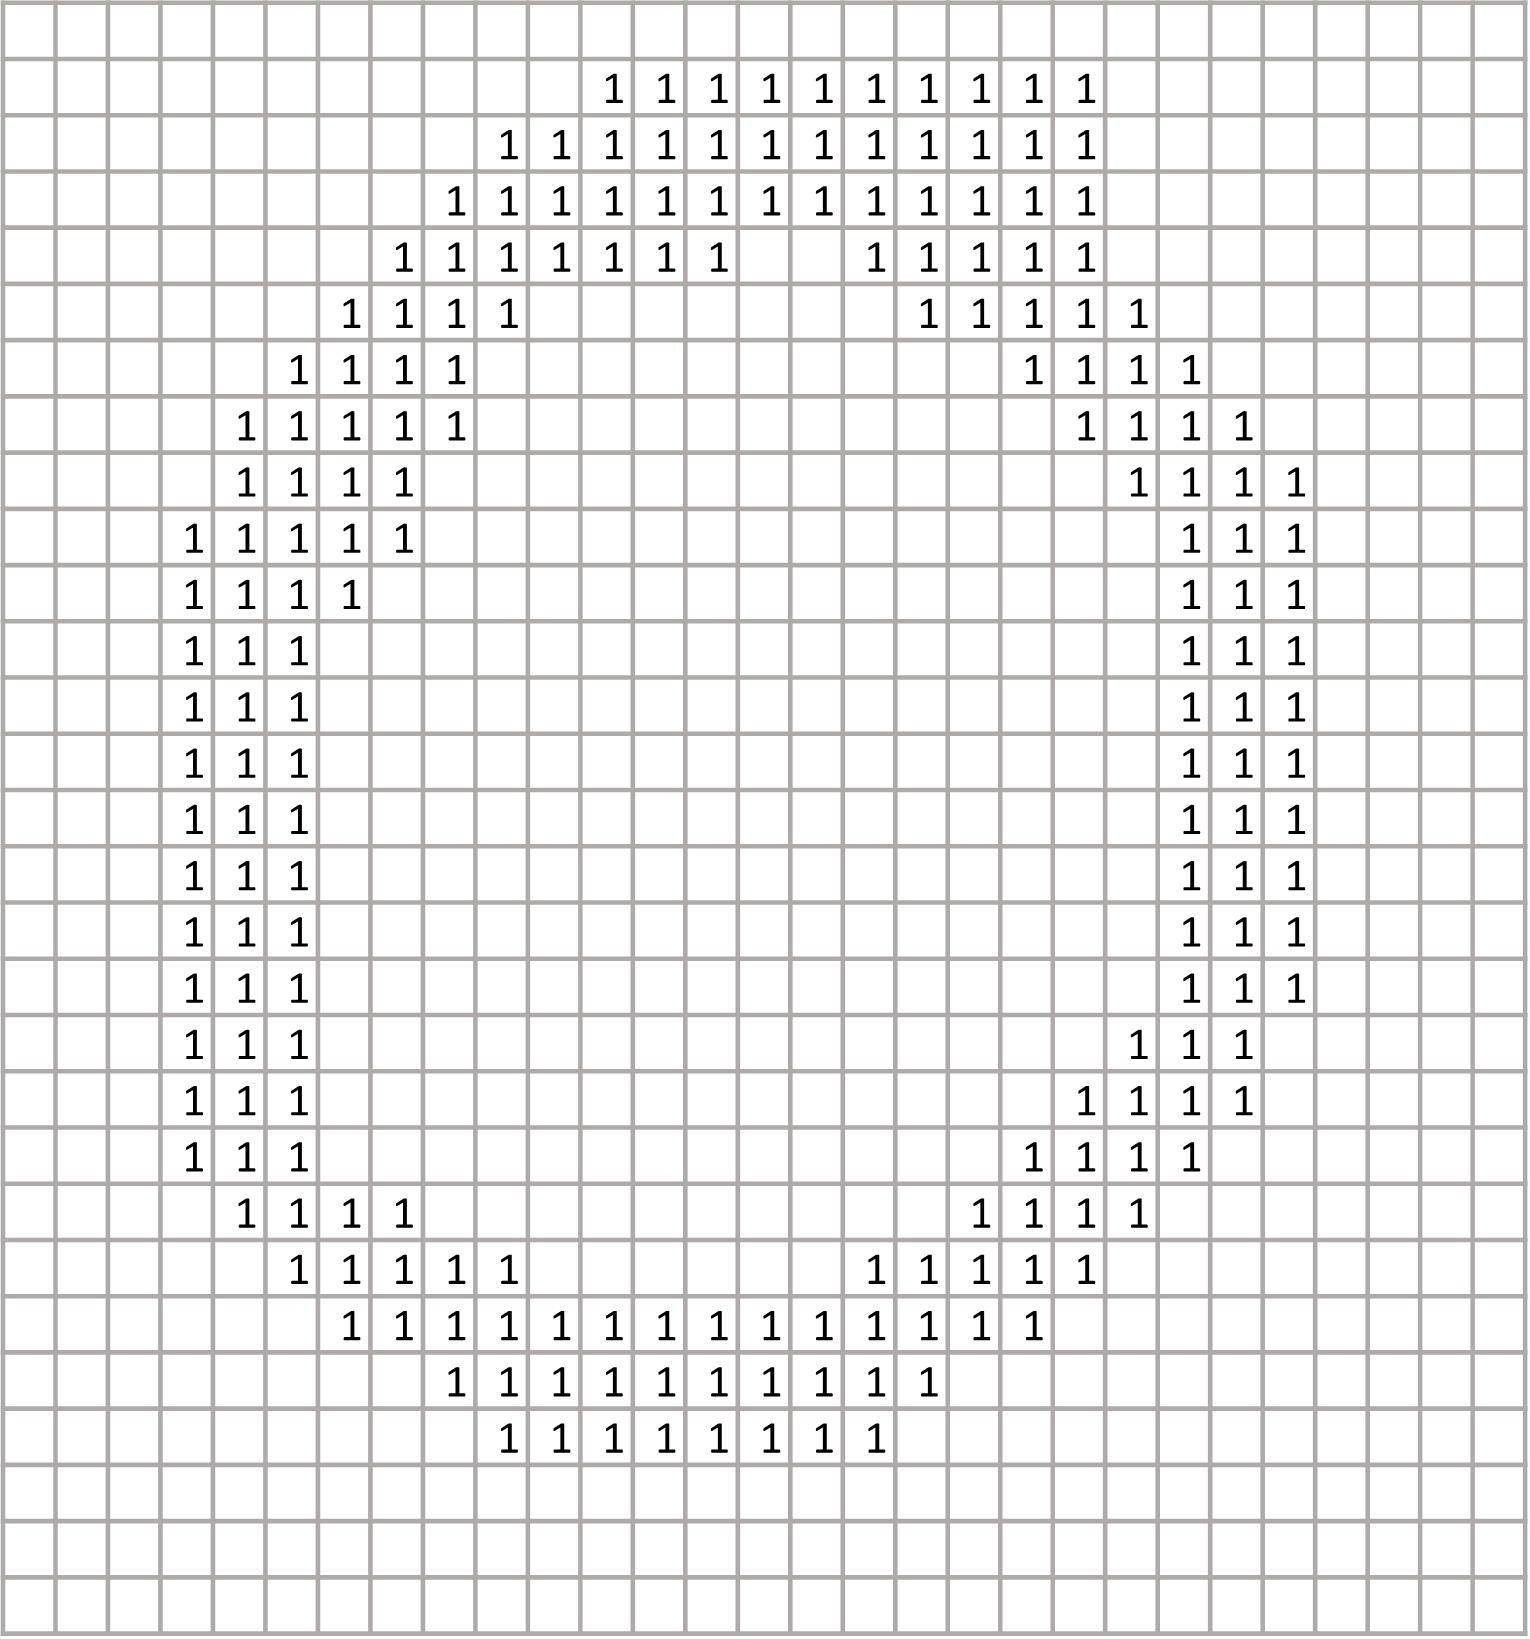
\includegraphics[width=.4\textwidth]{figuras/digito_0.png}
    \caption{Exemplo de matriz de uma imagem binária com dígito 0 onde os pixels pretos são representados por 1 e os pixels brancos são representados por 0. Os valores zero foram omitidos para uma melhor visualização.}
    \label{fig:dig_0}
\end{figure}

O problema de reconhecimento de dígitos possui naturalmente uma restrição de ser invariante por translação, uma vez que a classificação do dígito não deve depender de sua posição na imagem, por exemplo, se ele estiver centralizado ou deslocado do centro. Esta e outras restrições são feitas implicitamente pela representação paramétrica das hipóteses como WOMC para classificação de imagens de forma que o Espaço de Hipóteses é
$$\mathcal{H} = \left\{ h_{\theta} : \theta \in \Theta \right\}$$
sendo $h_{\theta} $ a hipótese com parâmetro $\theta \in \Theta$ definida por \eqref{eq:emolduradas}.

Por exemplo, assumindo que as imagens com os dígitos possuem tamanho $29 \times 29$, ou seja, $p = 29$ e $X \subseteq F_{29}$, e a janela $W$ tem tamanho $5 \times 5$, ou seja, $d_{W} = 5$ e $W \subseteq F_{5}$, temos que $n = 7$ e
$$ \theta_{fr} = \left\{ \left(W_{1}, f_{\psi_{1}^{fr}} \right), \cdot \cdot \cdot, \left(W_{7}, f_{\psi_{7}^{fr}} \right) \right\}$$
representará uma sequência fixa de sete W-operadores que gera o classificador
$$h_{\theta} := \left( \psi_{7}^{fr} \circ \psi_{6}^{fr} \circ \psi_{5}^{fr} \circ \psi_{4}^{fr} \circ \psi_{3}^{fr} \circ \psi_{2}^{fr} \circ \psi_{1}^{fr}  \right).$$

Então, após aplicar cada W-operador a dimensão da saída reduz em $4$ unidades e como $28 = p-1 = n \left( d_{W}-1 \right) = 7 \times 4$, após aplicar $7$ W-operadores em sequência, a dimensão da saída será $p - n \left( d_{W}-1 \right) = 29 - 28 = 1$, e $h_{\theta}$ terá imagem em $\left\{ 0,1 \right\}$. 


%%%%%%%%%%%%%%%%%%%%%%%%%%%%%%%%%%%%%%%%%%%%%%%%%%%%%%%%%%%%%%%%%%%%%%%%%%%%%%%%%%%
\section{Aprendizado de W-operadores Multicamadas}
\label{sec:aprendizado}

O aprendizado de W-operadores multicamadas no contexto de transformação ou de classificação de imagens é semelhante e será apresentado nesta seção. O algoritmo aprende de forma simultânea a janela e a função característica de todos os W-operadores.

\subsection{Amostras de Treino e Validação}

Para um valor fixo $p \in \mathbb{Z}_{+} $, seja $\mathcal{D}_{N} = \left\{ \left( X_{1}, Y_{1} \right),...,\left( X_{N}, Y_{N} \right) \right\} $ a amostra de treinamento de $N$ imagens de entrada emolduradas $X_{i} \subseteq F_{p} $ e suas correspondentes imagens de saída $Y_{i} \subseteq F_{q} $. No contexto de transformação de imagens assumimos que $q = p$ de forma que $Y_{i} \subseteq F_{p} $ é uma imagem emoldurada obtida pela transformação de $X_{i}$. Já no contexto de classificação de imagens assumimos que $q=1$ e $Y_{i} \in \mathcal{P} \left( \left\{ \left( 0,0 \right) \right\} \right) \simeq \left\{ 0,1 \right\} $ é a classe de $X_{i}$.

Quando $ Y_{i}, \ i = 1,...,N,$ são imagens emolduradas em $F_{p}$, denotamos para $ \left( j,k \right) \in F_{p} $ e $\theta \in \Theta$ como
$$\left( Y_{i} \right)_{j,k}$$
o valor do pixel $\left( j,k \right)$ na imagem $Y_{i}$ e 
$$ \left( \psi_{\theta} \left( X_{i} \right) \right)_{j,k} $$
o valor do pixel $\left( j,k \right)$ na imagem $\psi_{\theta} \left( X_{i} \right)$.

Seja $ \ell \left( \left( X_{i}, Y_{i} \right), \theta \right) \in \mathbb{R}_{+}$ o erro obtido quando o W-operador $ \psi_{\theta}$  é aplicado para transformar $X_{i}$ em $Y_{i}$, ou quando o classificador $h_{\theta}$ é utilizado para prever a classe $Y_{i}$ de $X_{i}$. Neste trabalho consideramos duas funções de perda quando $Y_{i}$ é uma imagem emoldurada em $F_{p}$, \textbf{MAE} dada por
$$ \ell_{MAE} \left( \left( X_{i}, Y_{i} \right), \theta \right) = \frac{1}{p^{2}} \sum_{(j,k) \in F_{p}} | \left( \psi_{\theta} \left( X_{i} \right) \right)_{j,k} - \left( Y_{i} \right)_{j,k} | $$
ou interseção sobre união (\textbf{IoU}) dada por
$$ \ell_{IoU} \left( \left( X_{i}, Y_{i} \right), \theta \right) = 1 - \frac{Y_{i} \cap \psi_{\theta} \left( X_{i} \right)}{Y_{i} \cup \psi_{\theta} \left( X_{i} \right)} $$
quando $Y_{i}$ é uma classe de $X_{i}$, utilizamos o erro \textbf{MAE} dado por
$$ \ell_{MAE} \left( \left( X_{i}, Y_{i} \right), \theta \right) = | h_{\theta} \left( X_{i} \right) - Y_{i} |. $$
O erro empírico de $\theta \in \Theta$ na amostra de treinamento $\mathcal{D}_{N}$ será então considerado como
$$ L_{t} \left( \theta \right) = \frac{1}{N} \sum_{i=1}^{N} \ell  \left( \left( X_{i}, Y_{i} \right), \theta \right). $$

No contexto de transformação de imagens, $L_{t}$ representa a proporção média de pixels com valores distintos em $Y_{i}$ e $\psi_{\theta} \left( X_{i} \right), \ i=1,...,N $ e, no contexto de classificação de imagens, $L_{t}$ representa o erro de classificação de $h_{\theta}$ na amostra $\mathcal{D}_{N}$.

Analogamente, temos a amostra de validação $\tilde{\mathcal{D}}_{M} = \left\{ \left( \tilde{X}_{1}, \tilde{Y}_{1} \right),...,\left( \tilde{X}_{M}, \tilde{Y}_{M} \right) \right\} $, que é independente de $\mathcal{D}_{N}$, cujo erro empírico é dado por
$$ L_{v} \left( \theta \right) = \frac{1}{M} \sum_{i=1}^{M} \ell  \left( \left( \tilde{X}_{i}, \tilde{Y}_{i} \right), \theta \right) $$
para $\theta \in \Theta$.

A partir deste ponto não faremos distinção entre o aprendizado de WOMC nos contextos de transformação e classificação de imagens, uma vez que são análogos, com a diferença no cálculo do erro empírico, conforme apresentado acima.

%%%%%%%%%%%%%%%%%%%%%%%%%%%%%%%%%%%%%%%%%%%%%%%%%%%%%%
\subsection{LS para o Aprendizado de W-operadores Multicamadas}

Para cada sequência de $n$ janelas $\textbf{W} = \left\{ W_{1},...,W_{n} \right\} \in \mathscr{C}^{n} $, denote a classe das sequências de W-operadores com janelas $\textbf{W}$ como
\begin{equation}
    \Theta_{\textbf{W}} := \left\{ \left\{ \left( W_{1}, f_{\psi_{1}} \right),..., \left( W_{n}, f_{\psi_{n}} \right) \right\} : f_{\psi_{i}} \in \mathcal{F}_{W_{i}}, i=1,...,n \right\}
    \label{eq:ThetaW}
\end{equation}

As sequências em $\Theta_{\textbf{W}}$ geram subespaços, ou modelos, de $\mathcal{H}$ dos W-operadores multicamadas emoldurados com janela $\textbf{W}$ definidos como
\begin{align*}
    \mathcal{M}_{\textbf{W}} := \left\{ h_{\theta} : \theta \in \Theta_{\textbf{W}} \right\}  & & \text{ ou } & & \mathcal{M}_{\textbf{W}} := \left\{ \psi_{\theta} : \theta \in \Theta_{\textbf{W}} \right\}.
\end{align*}
Esses modelos geram o LS cujos modelos são compostos pelos WOMC com cada possibilidade de sequência de janelas $\textbf{W}$, definido como
\begin{equation}
    \mathbb{L} \left( \mathcal{H} \right) = \left\{ \mathcal{M}_{\textbf{W}}: \textbf{W} \in \mathscr{C}^{n} \right\}.
    \label{eq:ls}
\end{equation}
O aprendizado dos WOMC será feito através do aprendizado nesse LS.

%%%%%%%%%%%%%%%%%%%%%%%%%%%%%%%%%%%%%%%%%%%%%%%%%%%%%%
\section{Algoritmo U-curve Para o Aprendizado de W-operadores Multicamadas}

O algoritmo U-curve \cite{REIS201997} para minimizar uma função em um subconjunto de um reticulado Booleano realiza uma busca gulosa no reticulado, de forma análoga ao algoritmo de gradiente descendente, e a cada etapa pula para um nó de distância um do nó atual e para quando todos os nós vizinhos tem um erro maior ou igual a este nó. Estes algoritmos são ótimos quando satisfazem a propriedade U-curve \cite{marcondes2021learning} e sub-ótimos quando não satisfazem, porém mesmo em casos sub-ótimos o algoritmo pode retornar um nó com erro pequeno o suficiente de forma eficiente, sem a necessidade da busca exaustiva no reticulado.

\subsection{Ideias Principais}
\label{subsec:alg_ideiasprinc}

O algoritmo U-curve para o aprendizado dos WOMC consiste basicamente de três etapas conforme descrito a seguir.

\begin{enumerate}
    \item \textbf{Inicialização do algoritmo} 
    \begin{enumerate}
        \item O tamanho máximo $d_{W}$ das janelas a serem treinadas bem como a quantidade $n$ de janelas são pré-definidos (no contexto de classificação $n$ é definido com base no tamanho das imagens de aprendizado);
        \item O elemento estruturante das janelas iniciais pode ser gerado de forma aleatória ou inicializado por uma janela pré-definida;
        \item A função característica das janelas iniciais são geradas aleatoriamente dado o elemento estruturante da respectiva janela.
    \end{enumerate}
    \item \textbf{Aprendizado do WOMC com janelas fixas}
    \begin{enumerate}
        \item Fixadas as janelas e as funções características, o \textit{batch size} b, o número $r$ de vizinhos a serem amostrados em cada camada, o número de épocas de treinamento e o \textit{early stop} $es_f$ são fixos. Calculamos então o erro inicial de treinamento do WOMC gerado por essas janelas e funções características, que será o erro do \textit{nó mínimo} inicial ou $L_{t_{min}}$;
        \item Para cada época, a amostra de treinamento é particionada aleatoriamente em $N/b$ lotes, e denotamos o erro de treinamento no \textit{batch} $j$ por $L_{t}^{(j)}$;
        \item para cada \textit{batch} sorteamos $r$ vizinhos de cada camada e um a um os bits desses vizinhos da função característica são invertidos, ou seja, um bit que era 0 se torna 1 e um bit que era 1 se torna 0;
        \item Para cada inversão calculamos o erro de treinamento $L_{t_{1}}^{(j)}, ..., L_{t_{d}}^{(j)}$ do WOMC obtido após a respectiva inversão, onde $d$ é o número máximo de inversões possíveis da função dada a quantidade de vizinhos da janela e o número de vizinhos sorteados $r$; 
        \item O algoritmo irá pular para a inversão com menor erro, ou seja $min \left(L_{t_{i}}^{(j)} \right), \ 1 \leq i \leq d$, e sua respectiva função característica e esta se tornará o \textit{nó atual};
        \item Ao final de uma época, quando o algorítimo tiver percorrido todos os \textit{batchs}, será calculado o erro total de treinamento com o novo nó atual $L_{t}$. Se este erro for menor que o erro mínimo, ou seja, $L_{t}< L_{t_{min}}$ o erro mínimo sera atualizado para o erro do nó atual e a função característica será armazenada como a função característica mínima;
        \item Os itens (b)-(c)-(d)-(e)-(f) se repetem até rodarmos todas as épocas pré-determinadas ou caso o algoritmo estiver a $es_f$ épocas sem diminuir o erro e assim o aprendizado do WOMC com janelas fixas é finalizado.
    \end{enumerate}
    \item \textbf{Aprendizado das janelas do WOMC}
    \begin{enumerate}
        \item Para uma sequência de janelas fixadas iniciais, o \textit{batch size} b, o número $s$ de vizinhos a serem amostrados em cada camada, o número de épocas de treinamento e o \textit{early stop} $es_w$ são fixos. Calculamos o erro na amostra de validação do WOMC aprendido em (2), que será o erro do \textit{nó mínimo} inicial ou $L_{v_{min}}$;
        \item Para cada época, a amostra de validação é particionada aleatoriamente em $M/b$ lotes, e denotamos o erro de treinamento no \textit{batch} $j$ por  $L_{v_{min}}^{(j)}$;
        \item Para cada \textit{batch} sorteamos $s$ vizinhos para cada camada e um a um adicionamos e retiramos um ponto do elemento estruturante das janelas desses vizinhos, garantindo que a janela obtida seja uma janela conectada (Figura \ref{fig:wconect});
        \item Para cada adição/remoção inicializamos de forma aleatória a função característica da janela que foi alterada;
        \item Realizamos um novo treinamento (item (2)) para cada adição/remoção e calculamos o erro de validação $L_{v_{1}}^{(j)}, ..., L_{v_{g}}^{(j)}$, onde $g$ é o número de adições/remoções máximas possíveis de um ponto, garantindo que a nova janela continue conectada, dependendo da quantidade de vizinhos dessa janela e da quantidade de vizinhos $s$ sorteados; 
        \item O algoritmo irá pular para a adições/remoção com menor erro, ou seja $min \left(L_{v_{i}}^{(j)} \right), \ 1 \leq i \leq g$, com a respectiva configuração de janelas $i$ e esta se tornará o \textit{nó atual};
        \item Ao final de uma época, quando o algorítimo tiver percorrido todos os \textit{batchs}, será calculado o erro total de validação com o novo nó atual $L_{v}$. Se este erro for menor que o erro mínimo, ou seja, $L_{v}< L_{v_{min}}$ , o erro mínimo sera atualizado para o erro do nó atual e a configuração de janelas será armazenada como mínima;
        \item Os itens (b)-(c)-(d)-(e)-(f)-(g) se repetem até rodarmos todas as épocas pré-determinadas ou caso o algoritmo estiver a $es_w$ épocas sem diminuir o erro e assim o aprendizado é finalizado, obtemos o WOMC treinado e o algoritmo é parado.
    \end{enumerate}
\end{enumerate}

As subseções a seguir irão detalhar formalmente as etapas (2) e (3) do algoritmo descrito.

\subsection{Aprendizado de W-operador Multicamada com Janelas Fixas}

Seja $\Theta_{\textbf{W}}$, definido na Equação \ref{eq:ThetaW}, a classe das sequências de W-operadores com janelas $\textbf{W}$, e seja
$$\hat{\theta}_{\textbf{W}}:= \underset{\theta \in \Theta_{\textbf{W}}}{\arg \min } \ L_{t} \left( \theta \right)$$
o WOMC em $\Theta_{\textbf{W}}$ com o menor erro empírico sob a amostra de treinamento $\mathcal{D}_{N}$.

O cálculo de $\hat{\theta}_{\textbf{W}}$ pode ser muito complexo, uma vez que, em principio, é necessário calcular o erro empírico de cada $\theta \in \Theta_{\textbf{W}}$, o que não é possível devida a alta cardinalidade de $\Theta_{\textbf{W}}$, uma vez que $|\Theta_{\textbf{W}}| = \prod_{i=1}^{n} 2^{|W_{i}|}$ é um número muito grande, mesmo para $n$ e $|W_{i}|$ pequenos.

Ao invés de minimizar o erro empírico, propomos um Algoritmo sub-ótimo que busca no reticulado Booleano um $\theta \in \Theta_{\textbf{W}}$ \textit{localmente bom} de acordo com a amostra de treinamento $\mathcal{D}_{N}$.

Para uma janela fixa $W \in \mathscr{C}$, denotamos $\mathscr{L}_{W} = \left\{ 0,1 \right\}^{\mathcal{P}(W)} $ e observamos uma bijeção entre $ \mathcal{F}_{W} $ e $\mathscr{L}_{W}$. Seja $ \left( \mathscr{L}_{W} , \leq \right)  $ um reticulado Booleano no qual, para $w, w' \in  \mathscr{L}_{W}$,
$$w \leq w' \iff w_{i}  \leq w'_{i}, \forall i = 1,...,2^{|W|}, $$
onde $ w_{i}, w'_{i} $ são as coordenadas de $ w, w'$. Da bijeção acima temos que $ \mathcal{F}_{W} $ é isomórfico a um reticulado Booleano.

Da mesma maneira, fixando $\textbf{W} \in \mathscr{C}^{n}$, denotamos $ \mathscr{L}_{\textbf{W}} =  \prod_{i=1}^{n} \left\{ 0,1 \right\}^{\mathcal{P}(W_{i})} $, e observamos uma bijeção entre $\mathscr{L}_{\textbf{W}}$ e $\Theta_{\textbf{W}}$. Seja $ \left( \mathscr{L}_{\textbf{W}} , \leq \right)  $ um reticulado Booleano no qual, para $\textbf{w}, \textbf{w'} \in  \mathscr{L}_{\textbf{W}}$,
$$\textbf{w} \leq \textbf{w'} \iff w_{j}  \leq w'_{j}, \forall j = 1,...,n, $$
ou seja, $\textbf{w}$ no produto cartesiano é menor ou igual a $\textbf{w'}$ se e somente se cada um dos seus elementos é menor ou igual ao elemento correspondente de $\textbf{w'}$ no respectivo reticulado Booleano. Por bijeção, consideramos o reticulado Booleano $\left( \Theta_{\textbf{W}}, \leq \right) $.

Definimos os mínimos locais fortes de $\left( \Theta_{\textbf{W}}, \leq \right) $ como os pontos em $\Theta_{\textbf{W}}$ com erro de treinamento menor ou igual a todos os pontos com distância um dele. Denotamos por $d$ a distância no grafo direcionado acíclico $\left( \Theta_{\textbf{W}}, \leq \right). $

\begin{definition}
    $\theta$ será um mínimo local forte de $\Theta_{\textbf{W}}$ sse
    $$ L_{t} \left( \theta \right) \leq \min \left\{ L_{t} \left( \theta' \right): \theta' \in \Theta_{\textbf{W}}, \ d \left( \theta,\theta' \right) = 1 \right\}. $$
\end{definition}

Observe que $\theta, \theta' \in \Theta_{\textbf{W}} $ são tais que $d \left( \theta,\theta' \right) = 1$ se e somente se suas funções características são iguais exceto por um ponto. Em outras palavras, $\theta'$ é obtido ao inverter a imagem de um ponto de uma função característica de $\theta$ de 0 para 1 ou de 1 para 0. Chamamos então formalmente de vizinho de $\theta$ como $N \left( \theta \right) = \{ \theta' \in  \Theta_{\textbf{W}}: d \left( \theta,\theta' \right) = 1 \}$. Estes são os casos de inversões descritas em \ref{subsec:alg_ideiasprinc} no item (2.c) da descrição informal do algoritmo. 

O algoritmo chamado \textit{Gradiente Descendente no Reticulado para o Aprendizado das Funções Características dos W-operadores Multicamadas com Janelas Fixas $\textbf{W} = \left\{ W_{1},...,W_{n} \right\} $} é apresentado no Algoritmo \ref{alg:graddescfunc}, e retorna $\theta_{\textbf{W}}^{\mathbb{A}}$, uma aproximação de $\hat{\theta}_{\textbf{W}}$. Esse algoritmo se refere a parte (2) da descrição informal da Seção \ref{subsec:alg_ideiasprinc}.

Vamos inserir no algoritmo \ref{alg:graddescfunc} duas fontes de estocasticidade realizando uma amostragem de vizinhos $N \left( \theta \right)$ a serem visitados e uma amostragem da imagens de treinamento $\mathcal{D}_{N}$ em lotes, chamadas de \textit{batch}. A estocasticidade é vantajosa por ter uma convergência mais rápida, pois atualizações mais frequentes podem acelerar a aproximação da solução ideal,  ter maior eficiência computacional ao visitar menos vizinhos e utilizando mini-lotes dos conjuntos de dados em cada iteração, principalmente quando o treinamento envolver grandes conjuntos de dados e janelas de W-operadores com maior complexidade e ter uma melhor generalização, dado que o modelo é constantemente exposto a diferentes subconjuntos dos dados, tornando-o mais robusto a variações nos dados de entrada.

Ao invés de parar no primeiro mínimo local, como em algoritmos tradicionais baseados em U-curve, vamos adotar uma abordagem de percorrer o reticulado booleano em épocas, devido a aleatoriedade inerente à estocasticidade, especialmente na seleção de vizinhos. Em cada época, ocorre a exposição completa dos dados, percorrendo todos os \textit{batchs}, porém em cada \textit{batch} andaremos um passo no reticulado, permitindo uma aproximação mais precisa da solução ótima. Além disso, empregamos o parâmetro de \textit{early stop} para otimizar o tempo de treinamento. Esse parâmetro interrompe o treinamento quando não há mais melhorias significativas no erro, economizando tempo e recursos computacionais ao evitar épocas desnecessárias de treinamento.

O algoritmo \ref{alg:graddescfunc} é então inicializado em um $\theta \in \Theta_{\textbf{W}}$ fixado. Quando esse algoritmo é aplicado para o primeiro nó das janelas, esse $\theta$ é aleatório, mas quando é aplicado para outras janelas, esse $\theta$ é obtido a partir das funções características das janelas anteriores. O \textit{batch size} $b$, o número $r$ de vizinhos a serem amostrados em cada etapa, o número de épocas de treinamento e o \textit{early stop} $es_f$ são fixos. O algoritmo então realiza uma busca gulosa em $\left( \Theta_{\textbf{W}}, \leq \right)$ percorrendo as épocas pré-estabelecidas. Para cada época, a amostra de treinamento é particionada aleatoriamente em $N/b$ lotes. Para cada \textit{batch}, são amostrados $r$ vizinhos de $\theta$, $\tilde{N}\left(\theta\right) $, tal que $\tilde{N}\left(\theta\right) \in N\left(\theta\right)$. $\theta$ é atualizado para o vizinho amostrado com o menor erro de treinamento, calculado no \textit{batch} $j$ pra as imagens particionadas nesse \textit{batch}. $\theta$ é atualizado em cada \textit{batch}, então durante uma época, ele é atualizado $N/b$ vezes. Ao final de cada época, o erro de treinamento $ L_{t}\left(\theta\right)$ de $\theta$ atual é calculado para toda a amostra de treinamento e comparado com o erro $ L_{t_{min}}$, ponto com o menor erro de treinamento visitado até o momento, caso ele seja menor,  $ L_{t_{min}}$ é atualizado, assim como $\theta_{\textbf{W}}^{\mathbb{A}}$ e $Epoch_{min}$. Caso o algoritmo esteja a $es_f$ sem diminuir o erro, ou seja $(\text{run} - Epoch_{min}) > es_f$, o algoritmo \ref{alg:graddescfunc} encerra retornando o ponto com menor erro de treinamento encontrado.

Observe que se $r := |N\left(\theta\right)|$ e se $b=N$ então o algoritmo se reduz à versão determinística. Ou seja, a complexidade do algoritmo é controlada pelo número $r$ de vizinhos amostrados, pelo tamanho do \textit{batch} $b$ e pelo número de épocas.

\begin{algorithm}
    \caption{\textit{Algoritmo Gradiente Descendente no Reticulado para o Aprendizado das Funções Características dos W-operadores Multicamadas com Janelas Fixas $\textbf{W} = \left\{ W_{1},...,W_{n} \right\} $}}\label{alg:graddescfunc}
    \begin{algorithmic}[1]
        \Ensure $ \theta \in \Theta_{\textbf{W}}, Epochs_{f}, b, r, es_f $
        \State $L_{t_{min}}\leftarrow L_{t} \left( \theta \right)$
        \State $\theta_{\textbf{W}}^{\mathbb{A}} \gets \theta$
        \State $Epoch_{min} \leftarrow 0$
        \For{$\text{run} \in \{1,..., Epochs_{f}\}$} 
            \State ShuffleBatches($b$)
            \For{$j \in \{1,...,N/b\}$}
                \State $\tilde{N} \left(\theta\right) \leftarrow \text{SampleNeighbors}\left(\theta,r\right)$
                \State $\theta \leftarrow \theta'$ s.t. $\theta' \in \tilde{N}\left(\theta\right)$ and $L_{t}^{\left(j\right)}\left(\theta'\right) = \min\{L_{t}^{\left(j\right)}\left(\theta''\right):\theta'' \in \tilde{N}\left(\theta\right) \}$
            \EndFor
            \If{$ L_{t} \left( \theta \right) < L_{t_{min}}$}
                \State $L_{t_{min}}\leftarrow L_{t} \left( \theta \right)$
                \State $\theta_{\textbf{W}}^{\mathbb{A}} \gets \theta$
                \State $Epoch_{min} \leftarrow \text{run}$
            \EndIf
            \If{$(\text{run} - Epoch_{min}) > es_f$}
                \State \textbf{break}
            \EndIf
        \EndFor
        \State \textbf{return} $\theta_{\textbf{W}}^{\mathbb{A}}$
    \end{algorithmic}
\end{algorithm}

\subsection{Aprendizado das Janelas do W-operador Multicamada}

Para aprendermos as janelas de um WOMC tammbém aplicamos o Algoritmo do Gradiente Descendente no Reticulado em $\mathscr{C}^{n}$ (Algoritmo \ref{alg:graddescjan}), que é um subconjunto de um reticulado Booleano. 

Considere a ordem parcial em $\mathscr{C}^{n}$ dada por
\begin{equation}
    \textbf{W} \leq \textbf{W}' \iff W_{i} \subseteq W'_{i}, \ \text{para todo } i=1,...,n.
    \label{eq:Worder}
\end{equation}
Uma vez que cada $W_{i}$ é um subconjunto de $F_{d_{W}}$, então $\mathscr{C}^{n} $ é um subconjunto de
$$\prod_{i=1}^{n} \left\{ 0,1 \right\}^{F_{d_{W}}} $$
que é um reticulado Booleano com ordem parcial equivalente a \eqref{eq:Worder}.

Para cada $\textbf{W} \in \mathscr{C}^{n} $, seja
$$ \hat{L} \left( \textbf{W} \right) := L_{v} \left( \theta_{\textbf{W}}^{\mathbb{A}} \right)$$
o erro empírico da amostra de validação do WOMC $\theta_{\textbf{W}}^{\mathbb{A}}$ retornado pelo Algoritmo \ref{alg:graddescfunc}. A escolha de janelas seria
$$\hat{\textbf{W}} := \underset{\textbf{W} \in \mathscr{C}^{n}}{\arg \min } \ \hat{L} \left( \textbf{W} \right), $$
que é a janela $\textbf{W}$ tal que $\theta_{\textbf{W}}^{\mathbb{A}}$ tem o menor erro empírico sob a amostra de validação. No entanto, como no aprendizado das funções características de um WOMC com janelas fixas, o cálculo de $\hat{\textbf{W}} $ é inviável e devemos considerar uma solução sub-ótima.

Ao invés de $\hat{\textbf{W}} $, iremos aprender a sequência de janelas encontrando um mínimo local forte de $\hat{L}$ em $\mathscr{C}^{n}$ pelo \textit{Algoritmo Gradiente Descendente no Reticulado para o Aprendizado das Janelas dos W-operadores Multicamadas} \ref{alg:graddescjan}. Definimos os mínimos locais fortes de $\mathscr{C}^{n}$ em \ref{def:minC}, onde $d$ é a distância no grafo direcionado acíclico $\left( \mathscr{C}^{n}, \leq \right) $.

\begin{definition}
    $\textbf{W}$ será um mínimo local forte de $\mathscr{C}^{n}$ sse
    $$\hat{L} \left( \textbf{W} \right) \leq \min \left\{ \hat{L} \left( \textbf{W} ' \right): \textbf{W} ' \in \mathscr{C}^{n}, \ d \left( \textbf{W} ,\textbf{W}' \right) = 1 \right\} $$
    \label{def:minC}
\end{definition}

Observe que $\textbf{W} ,\textbf{W}' \in \mathscr{C}^{n} $ são tais que $d \left(\textbf{W} ,\textbf{W}' \right) = 1$ se e somente se suas janelas são iguais exceto por um ponto. Em outras palavras, $\textbf{W}'$ é obtido ao adicionar ou remover um ponto do elemento estruturante de $\textbf{W}$. Chamamos então formalmente de vizinho de $\textbf{W}$ como $N \left( \textbf{W} \right) = \{ \textbf{W}'  \in \mathscr{C}^{n}: d \left( \textbf{W} ,\textbf{W}' \right) = 1 \}$ Estes são os casos de adição/remoção descritas em \ref{subsec:alg_ideiasprinc} no item (3.b) da descrição informal do algoritmo.

O algoritmo chamado \textit{Gradiente Descendente no Reticulado para o Aprendizado das Janelas dos W-operadores Multicamadas}  apresentado no Algoritmo \ref{alg:graddescjan} retorna $\textbf{W}^{\mathbb{A}}$, uma aproximação de $\hat{\textbf{W}}$. Esse algoritmo se refere a parte (3) da descrição informal da Seção \ref{subsec:alg_ideiasprinc}.

Assim como no Algoritmo \ref{alg:graddescfunc}, o Algoritmo \ref{alg:graddescjan} possui duas fontes de estocasticidade realizando uma amostragem de vizinhos $N\left( \textbf{W} \right)$ a serem visitados e uma amostragem em  \textit{batch} das imagens de validação $\tilde{\mathcal{D}}_{M}$. Também utiliza a abordagem de épocas para percorrer o reticulado e \textit{early stop} para encerrar o algoritmo quando não há diminuição do erro.

O algoritmo  é inicializado com o primeiro retorno do Algoritmo \ref{alg:graddescfunc} com Janela $\textbf{W} \in \mathscr{C}^{n}$ e WOMC $\theta_{\textbf{W}}^{\mathbb{A}}$. O \textit{batch size} $b$, o número $s$ de vizinhos a serem amostrados em cada etapa, o número de épocas de validação e o \textit{early stop} $es_w$ são fixos. O Algoritmo então realiza uma busca gulosa em $\left( \mathscr{C}^{n}, \leq \right) $ percorrendo as épocas pré-estabelecidas. Para cada época, a amostra de validação é particionada aleatoriamente em $M/b$ lotes. Para cada \textit{batch}, são amostrados $s$ vizinhos de $\textbf{W}$, $\tilde{N}\left(\textbf{W}\right) $, tal que $\tilde{N}\left(\textbf{W}\right) \in N\left(\textbf{W}\right)$. Para cada janela que teve seu elemento estruturante modificado, iremos gerar de forma aleatória a função característica da janela que foi alterada, e a função característica das demais janelas se manterão iguais, e chamaremos novamente o Algoritmo \ref{alg:graddescfunc} para encontrar $\theta_{\textbf{W'}}^{\mathbb{A}}$.

$\textbf{W}$ é atualizado para o vizinho amostrado com o menor erro de validação, calculado no \textit{batch} $j$ pra as imagens particionadas nesse \textit{batch}. $\textbf{W}$ é atualizado em cada \textit{batch}, então durante uma época, ele é atualizado $M/b$ vezes. Ao final de cada época, o erro de validação de $\textbf{W}$ atual é calculado para toda a amostra de validação e comparado com o erro $ L_{v_{min}}$, ponto com o menor erro de validação visitado até o momento, caso ele seja menor,  $ L_{v_{min}}$ é atualizado, assim como $\textbf{W}^{\mathbb{A}}$ e $Epoch_{min}$. Caso o algoritmo esteja a $es_w$ sem diminuir o erro, ou seja $(\text{run} - Epoch_{min}) > es_w$, o algoritmo \ref{alg:graddescjan} encerra retornando o ponto com menor erro de validação encontrado e o aprendizado é finalizado.

Podemos reparar que os algoritmos \ref{alg:graddescfunc} e \ref{alg:graddescjan} são análogos e diferem apenas no reticulado ($ \Theta_{\textbf{W}}$ e $ \mathscr{C}^{n}$) que percorrem e a função de erro que eles buscam minimizar (Erro de Treinamento e Validação)

\begin{algorithm}
    \caption{\textit{Algoritmo Gradiente Descendente no Reticulado para o Aprendizado das Janelas dos W-operadores Multicamadas}}\label{alg:graddescjan}
    \begin{algorithmic}[1]
        \Ensure $ \textbf{W} \in \mathscr{C}^{n},  Epochs_{w}, b, s, es_w $
        \State $L_{v_{min}}\leftarrow \hat{L} \left( \textbf{W} \right)$
        \State $\textbf{W}^{\mathbb{A}} \gets \textbf{W}$
        \State $Epoch_{min} \leftarrow 0$
        \For{$\text{run} \in \{1,..., Epochs_{w}\}$} 
            \State ShuffleBatches($b$)
            \For{$j \in \{1,...,M/b\}$}
                \State $\tilde{N} \left(\textbf{W}\right) \leftarrow \text{SampleNeighbors}\left(\textbf{W},s\right)$
                \State $\textbf{W} \leftarrow \textbf{W}'$ s.t. $\textbf{W}' \in \tilde{N}\left(\textbf{W}\right)$ and $ \hat{L}^{\left(j\right)} \left( \textbf{W}' \right) = \min \left\{  \hat{L}^{\left(j\right)} \left( \textbf{W}'' \right): \textbf{W}'' \in \tilde{N}\left(\textbf{W}\right) \right\} $
            \EndFor
            \If{$  \hat{L} \left( \textbf{W} \right) < L_{v_{min}}$}
                \State $L_{v_{min}}\leftarrow  \hat{L} \left( \textbf{W} \right)$
                \State $\textbf{W}^{\mathbb{A}} \gets \textbf{W}$
                \State $Epoch_{min} \leftarrow \text{run}$
            \EndIf
            \If{$(\text{run} - Epoch_{min}) > es_w$}
                \State \textbf{break}
            \EndIf
        \EndFor
        \State \textbf{return} $\theta_{\textbf{W}}^{\mathbb{A}}$
    \end{algorithmic}
\end{algorithm}

